\documentclass[tikz,border=8pt]{standalone}
\usepackage{amsmath}
\usepackage{pgfplots}
\pgfplotsset{compat=1.18}
\definecolor{ink}{HTML}{21352F}
\definecolor{teal}{HTML}{087F7B}
\definecolor{blue}{HTML}{4B77A8}
\definecolor{gold}{HTML}{C58B2A}
\definecolor{rose}{HTML}{B65A62}
\begin{document}
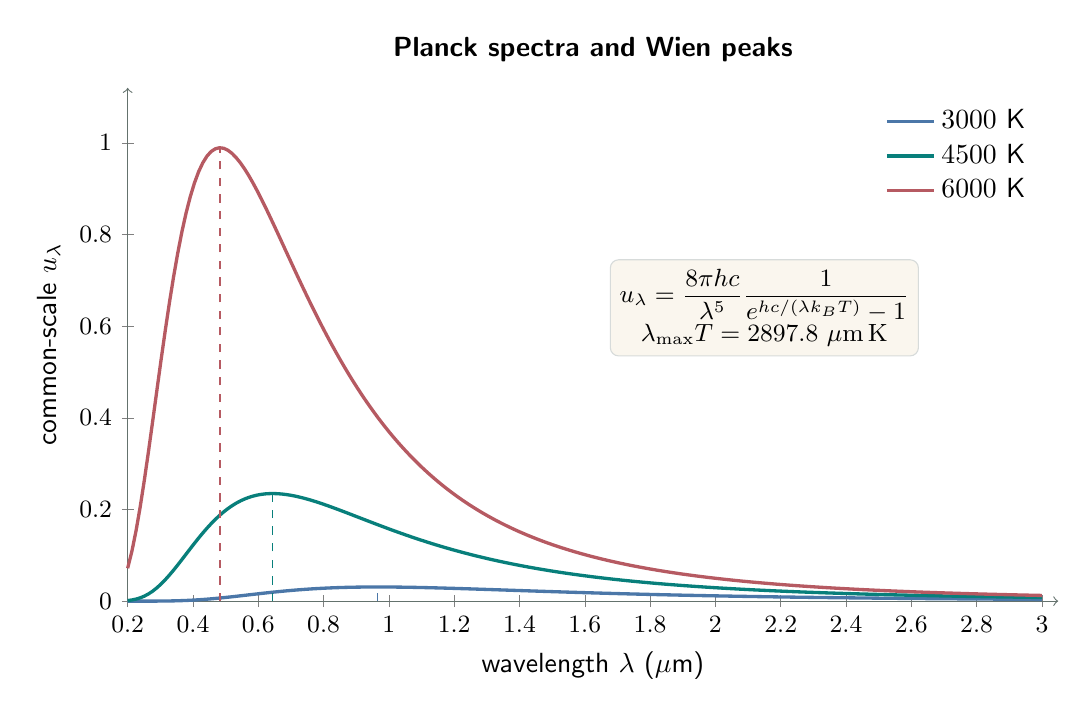
\begin{tikzpicture}[font=\sffamily]
\begin{axis}[
  width=13.4cm,height=8.1cm,
  xmin=.2,xmax=3.05,ymin=0,ymax=1.12,
  axis lines=left,
  axis line style={draw=ink!70,->},
  xlabel={wavelength $\lambda$ ($\mu$m)},
  ylabel={common-scale $u_\lambda$},
  title={\bfseries Planck spectra and Wien peaks},
  legend style={draw=none,fill=none,at={(.98,.98)},anchor=north east},
  tick label style={font=\small},
  clip=false
]
  \addplot[blue,very thick,domain=.2:3,samples=220]
    {3.7/(x^5*(exp(14387.77/(x*3000))-1))};
  \addlegendentry{$3000$ K}
  \addplot[teal,very thick,domain=.2:3,samples=220]
    {3.7/(x^5*(exp(14387.77/(x*4500))-1))};
  \addlegendentry{$4500$ K}
  \addplot[rose,very thick,domain=.2:3,samples=220]
    {3.7/(x^5*(exp(14387.77/(x*6000))-1))};
  \addlegendentry{$6000$ K}
  \pgfmathsetmacro{\xA}{2897.8/3000}
  \pgfmathsetmacro{\yA}{3.7/(\xA^5*(exp(14387.77/(\xA*3000))-1))}
  \pgfmathsetmacro{\xB}{2897.8/4500}
  \pgfmathsetmacro{\yB}{3.7/(\xB^5*(exp(14387.77/(\xB*4500))-1))}
  \pgfmathsetmacro{\xC}{2897.8/6000}
  \pgfmathsetmacro{\yC}{3.7/(\xC^5*(exp(14387.77/(\xC*6000))-1))}
  \addplot[blue,dashed] coordinates {(\xA,0) (\xA,\yA)};
  \addplot[teal,dashed] coordinates {(\xB,0) (\xB,\yB)};
  \addplot[rose,dashed] coordinates {(\xC,0) (\xC,\yC)};
  \node[draw=ink!18,fill=gold!8,rounded corners=3pt,
        font=\small,align=center] at (axis cs:2.15,.64)
    {$\displaystyle u_\lambda=
      \frac{8\pi hc}{\lambda^5}
      \frac1{e^{hc/(\lambda k_BT)}-1}$\\
     $\lambda_{\max}T=2897.8\ \mu{\rm m\,K}$};
\end{axis}
\end{tikzpicture}
\end{document}
